%!TEX root=../ends.tex
\section{The nerve and realization paradigm.}\label{section:nr}
\subsection{The classical nerve and realization.}
The most fruitful application of the machinery of Kan extensions is the ``Kan construction'' for the geometric \emph{realization} of simplicial sets as a topological space, or more precisely as a \textsc{cw}-complex. It is impossible to underestimate the value of this construction as a unification tool in algebra and algebraic topology; here, we briefly sketch this construction. This section assumes a certain acquaintance with the basic definition on simplicial homotopy theory; in particular, we take for granted the first chapter of \cite{GoJ} and the definition of a \emph{Quillen model category}.

Consider the category $\bDelta$ of finite nonempty ordinals and monotone functions, as  defined in \cite{GoJ}, and let us consider the Yoneda embedding $\yon_\Delta \colon \bDelta \to [\bDelta^\opp,\Sets]=\cate{sSet}$; we can define two functors $\rho\colon \bDelta\to \Top $ and $i\colon \bDelta\to \Cat$ which ``represent'' every object $[n]\in\bDelta$ either as a topological space or as a small category:
\begin{itemize}
\item The category $i[n]$ is $\{0\to 1\to\dots\to n\}$ (there is a similar functor $\cate{Pos}\to \Cat$ regarding any poset $(P,\le)$ as the category $\cate P$ where the composition function is induced by the partial order relation $\le$: $i$ here coincides with its restriction to $\bDelta\subset \cate{Pos}$);
\item The topological space $\rho[n]$ is defined as the \emph{standard $n$-simplex} $\Delta^n$ embedded in $\mathbb{R}^{n+1}$, 
\[
\rho[n] = \Big\{(x_0, \dots, x_n) \in \mathbb{R}^{n+1} \mid 0\leq x_i \leq 1, \textstyle \sum_{i=0}^n x_i = 1 \Big\}.
\]
\end{itemize}
In a few words, we are in the situation depicted by the following diagrams:
\[
\xymatrix{
\bDelta \ar[r]^i\ar[d]_{\yon_{\bDelta}} & \Cat \\
\cate{sSet}
}\qquad 
\xymatrix{
\bDelta \ar[r]^\rho\ar[d]_{\yon_{\bDelta}}& \Top \\
\cate{sSet}
}
\]
The two functors $i,\rho$ can be (left) Kan-extended along the Yoneda embedding $\yon_\Delta\colon \bDelta \to \sSet$, and these extensions happen to be left adjoints (this can be proved directly, but we will present in a while a completely general statement).

We denote these adjunctions
\[
\Lan_\yon i\dashv N_i \quad\text{ and }\quad \Lan_\yon \rho\dashv N_\rho;
\] 
these two right adjoint functors are called the \emph{nerves} associated to $i$ and $\rho$ respectively, and are defined, respectively, sending a category $\C$ to the simplicial set $N_i(\C)\colon [n]\mapsto \Cat(i[n],\C)$ (the \emph{classical nerve} of a category), and to the simplicial set $N_\rho(X)\colon[n]\mapsto \Top(\rho[n], X) = \Top(\Delta^n, X)$ (the \emph{singular complex} of a space $X$).\footnote{The name is motivated by the fact that if we consider the free-abelian group on $N_\rho(X)_n$, the various $C_n = \Z\cdot N_\rho(X)_n = \coprod_{ N_\rho(X)_n}\Z$ organize as a chain complex, whose homology is precisely the singular homology of $X$.}

The left adjoints to $N_\rho$ and $N_i$ must be thought as ``realizations'' of a simplicial set as an object of $\Top$ or $\Cat$:
\begin{itemize}
\item The left Kan extension $\Lan_\yon \rho$ is called the \emph{geometric} realization $|X_\bullet|$ of a simplicial set $X_\bullet$, and it can be characterized as the coend
\[
\int^{n\in\bDelta} \Delta^n \times X_n
\]
which in turn coincides to a suitable coequalizer in $\Top$ in view of our \refbf{coends.as.colims} and \refbf{endsareeq} (and their duals). 

The shape of this object is fairly easy to motivate, keeping open any book in algebraic topology: the topological space $|X_\bullet|$ is obtained choosing a $n$-dimensional disk $\Delta^n$ for each $n$-simplex $x \in X_n$ and gluing these disks along the boundaries $\delta_i(\Delta^n)$ according to the degeneracy maps of $X_\bullet$. The resulting space is (almost by definition) a \textsc{cw}-complex, because each standard $n$-simplex is homeomorphic to a closed disk: this means that  $|X_\bullet|$ has the topology induced by a sequential colimit of pushouts of spaces $X_{(0)} \to X_{(1)} \to\dots$
\item The left Kan extension$\Lan_\yon i$ is the \emph{categorical} realization $\tau_1(X_\bullet)$ of a simplicial set $X_\bullet$, resulting as the coend
\[
\int^{n\in\bDelta} i[n] \times X_n.
\]
This is the category whose objects are 0-simplices of $X_\bullet$, arrows are 1-simplices, and where composition is defined asking that $f,g\in X_1$ compose if there exists a 2-simplex $\sigma$ having 0-th face $g$ and 2-nd face $f$; identities are witnessed by degenerate simplices.% The category $i[n]$ can be regarded as the ``universal composable string of $n$ arrows'', and the action of degeneracies (given by composition of contiguous arrows) induces a composition law for $n$-tuples of arrows under the quotient that defines the coend.
\end{itemize}
We leave the reader think about why we only mention degeneracies here, leaving out faces (they are necessary, aren't they?).%, and we depict the geometric realization of $X_\bullet$ in figure~\refbf{fig:realiz}.
% \begin{center}
% \begin{figure}[h!]
% \begin{tikzpicture}[scale=.6]
% \fill (0,0)   circle (2pt) node (A) {};
% \fill (1,2)   circle (2pt) node (B) {};
% \fill (.5,-1) circle (2pt) node (C) {};
% \fill (3,0)   circle (2pt) node (D) {};
% \begin{scope}[xshift=5cm]
% \draw[thick] (0,0) node (A'2) {}-- (2,3.5) node (A2) {};
% \draw[thick] (1.15,0) node (B'2) {} -- (3.15,3.5) node (B2) {};
% \draw[thick] (45:.5) node (C'2) {} -- (45:2.5) node (C2) {};
% \draw[thick] (75:.5)  node (D'2) {} -- (75:4.5) node (D2) {};
% \end{scope}
% \begin{scope}[xshift=10cm]
% \draw[thick] (0,0) node (X1) {} -- (45:2.5) node (Y1) {} -- (2.5,0) node (Z1) {} -- cycle;
% \draw[thick] (3,3) node (X2) {} -- +(45:2.5) node (Y2) {} -- +(2.5,-1) node (Z2) {} -- cycle;
% \end{scope}
% \draw[->,dashed,black!90] (A) to [bend left] (A2);
% \draw[->,dashed,black!90] (C) to [bend left] (B'2);
% \draw[->,dashed,black!90] (B) to [bend left] (B2);
% %
% \draw[->,dashed,black!80] (A2) to [bend left] (Y2);
% \draw[->,dashed,black!80] (A'2) to [bend right=60] (Z2);
% \draw[->,dashed,black!80] (C'2) to [bend left] (Z1);
% \draw[->,dashed,black!80] (C2) to [bend left] (Y1);
% \draw[->,dashed,black!80] (B'2) to [bend left] (X1);
% \draw[->,dashed,black!80] (B2) to [bend left] (Y1);
% \end{tikzpicture}
% \label{fig:realiz}
% \caption{The construction of the geometric realization of $X \in \sSet$ as a sequential colimit of pushouts of disks.}
% \end{figure}
% \end{center}

It should now be evident that there is a pattern (we will call it the  ``nerve\hyp{}realization paradigm'') acting behind the scenes, and yielding the classical/singular nerve as particular cases of a general construction interpreted from time to time in different settings; unraveling this machinery with the power of co/end calculus is the scope of the following section.
\subsection{Some famous realizations and their associated nerves.}
Algebraic topology, representation theory, and more generally every setting where a well\hyp{}behaved categorical structure is involved constitute natural factories for examples of the nerve\hyp{}realization paradigm. We now want to lay down an foundation for a theory and a terminology that allows us to collect readable and enlightening examples (leaving outside many interesting others!) of nerve\hyp{}realizations pairs, obtained varying the domain category of ``geometric shapes'' or the category where this fundamental shapes are realized. 
\begin{definition}[context for nerve-realization]\label{nr-para}
Any functor $\varphi\colon \C\to \D$ from a small category $\C$ to a (locally small) \emph{cocomplete} category $\D$ is called a \emph{nerve\hyp{}realization context} (a \textsc{nr}\emph{-context} for short).
\end{definition}
Given a nerve\hyp{}realization context $\varphi$, we can prove the following result:
\begin{proposition}[Nerve-realization paradigm]\label{nervereal}
The left Kan extension of $\varphi$ along the Yoneda embedding $\yon \colon \C\to [\C^\opp, \Sets]$, \ie the functor $R_\varphi=\Lan_\yon \varphi\colon [\C^\opp, \Sets]\to \D$ is a left adjoint, $R_\varphi\dashv N_\varphi$. $R_\varphi$ is called the $\D$-\emph{realization functor} or the \emph{Yoneda extension} of $\varphi$, and its right adjoint the $\D$-\emph{coherent nerve}.
\end{proposition} 
\begin{proof}
The cocomplete category $\D$ is $\Sets$-tensored, and hence $\Lan_\yon \varphi$ can be written as the coend in equation (\refbf{kanend}); so the claim follows from the chain of isomorphisms
\begin{align*}
\D\big( \Lan_\yon \varphi(P),d \big)&\cong \D\Big(\int^c [\C^\opp,\Set](\yon_c,P)\cdot \varphi c,d \Big)\\
&\cong \int_c\D\big( [\C^\opp,\Set](\yon_c,P)\cdot \varphi c,d \big)\\
&\cong \int_c\cate{Sets}\big( [\C^\opp,\Set](\yon_c,P),\D(\varphi c,d) \big)\\
&\cong \int_c\Sets\big(Pc, \D(\varphi c,d)\big).
\end{align*}
If we define $N_\varphi(d)$ to be $c\mapsto \D(\varphi c,d)$, this last set becomes canonically isomorphic to $[\C^\opp,\Set](P,N_\varphi(d))$.
\end{proof}
It is straightforward to recognize $N_\rho$ and $N_i$ here.
\begin{remark}
The nerve\hyp{}realization paradigm can be rewritten in the following equivalent form: there is an equivalence of categories, induced by the universal property of the Yoneda embedding $\yon_\C : \C \to [\C^\opp,\Sets]$, 
\[
\yon_\C^* : \Cat(\C, \D)\cong \text{RAdj}(\widehat{\C}, \D)
\]
whenever $\D$ is a cocomplete locally small category (in such a way that ``the category of nerve\hyp{}realization contexts'' is a high-sounding name for the category of functors $\Cat(\C, \D)$).
\end{remark}
A famous result in Algebraic Topology \cite{GZ, GoJ} asserts that the geometric realization functor $R=|\firstblank| \colon \sSet\to\Top $ commutes with finite products: coend calculus gives a massive simplification of this result reducing it to the verification of the statement on representables only, but unfortunately
% .
% The main point of the proof is showing that the geometric realization commutes with products \emph{of representables}: the rest of the proof relies on a suitable application of coend-fu. We could appeal conceptual ways to show this preliminary result (\cite[\S \textbf{2}]{adamek2002classification}):
% \begin{proposition}\label{cofiltness}
% The following properties for a functor $F\colon \C\to \Sets$ are equivalent:
% \begin{itemize}
% \item $F$ commutes with finite limits;
% \item $\Lan_\yon F$ commutes with finite limits;
% \item $F$ is a filtered colimit of representable functors;
% \item The \emph{category of elements} $\elts{\C}{F}$ of $F$ (see Def\@. \refbf{eltsf} and Prop\@. \refbf{elementi}) is cofiltered.
% \end{itemize}
% \end{proposition}
isn't powerful enough to provide an additional simplification: formally, we can only define a \emph{bijection} between the sets $|\Delta[n]\times \Delta[m]|\cong \Delta^n \times \Delta^m$; a certain amount of dirty work is necessary to show that this bijection is in fact a homeomorphism with respect to the natural topologies on the two sets. 
\begin{proof}
If we take the commutativity of $R$ with finite products of representables for granted, the proof that $R(X\times Y)\cong RX\times RY$ is a simple computation:
% \begin{itemize}
% \item The geometric realization is a left adjoint, hence it commutes with colimits and tensors;
% \item Every simplicial set is a colimit of representables.
% \end{itemize}
% Starting the usual machinery, we have that
\begin{align*}
R( X\times  Y) &\cong \textstyle R\left[ \left(\int^m X_m\cdot \Delta[m] \right )\times \left( \int^n Y_n\cdot \Delta[n]\right ) \right ]\\
&\cong\textstyle R\left[ \int^{mn} (X_m\cdot \Delta[m])\times (Y_n\cdot \Delta[n])\right]\\
&\cong\textstyle R\left[\int^{mn} (X_m\times Y_n)\cdot (\Delta[m]\times \Delta[n]) \right ]\\
&\cong\textstyle \int^{mn}(X_m\times Y_n)\cdot R(\Delta[m]\times \Delta[n])\\
&\cong\textstyle \int^{mn}(X_m\times Y_n)\cdot \Delta^m\times\Delta^n \\
&\cong\textstyle \int^{mn} (X_m\cdot\Delta^m)\times (Y_n\cdot \Delta^n)\\
&\cong\textstyle \left(\int^mX_m\cdot\Delta^m\right)\times \left(\int^n Y_n\cdot \Delta^n \right )\\
&\cong  R( X)\times R( Y)
\end{align*}
where we applied, respectively, the ninja Yoneda lemma \refbf{ninjayo}, the colimit preservation property of $R$, its commutation with tensors, and its commutativity with finite products of representables.
\end{proof}
\subsection{Examples of nerves and realizations}
A natural factory of nerve\hyp{}realization contexts is \emph{homotopical algebra}, as such functors are often used to build Quillen equivalences between model categories. This is somewhat related to the fact that ``transfer theorem'' for model structures often apply to the well-behaved nerve functor.

But Quillen adjunctions between model categories are certainly not the only examples of \textsc{nr}-paradigms!

The following list attempts to gather important examples of \textsc{nr}-contexts: for the sake of completeness, we repeat the description of the two above-mentioned examples of the topological and categorical realizations.
\begin{example}[Categorical nerve and realization]\label{catnerve}
In the case of $\phi = i \colon \bDelta\to \Cat$, we obtain the \emph{classical nerve} $N_i$ of a (small) category $\C$, whose left adjoint is the \emph{categorical realization} (the \emph{fundamental category} $\tau_1 X$ of $X$ described in \cite{joyal2002quasi}). The nerve\hyp{}realization adjunction
\[
\tau_1 \colon \cate{sSet}\leftrightarrows \Cat\colon N_i
\]
gives a Quillen adjunction between the Joyal model structure on $\cate{sSet}$ (see \cite{joyal2002quasi}) and the folk model structure on $\Cat$.
\end{example}
\begin{example}[Geometric nerve and realization]\label{topnerve} 
If $\varphi = \rho \colon\bDelta\to \Top$ is the realization of a representable $[n]$ in the standard topological simplex, we obtain the adjunction between the \emph{geometric realization} $|X|$ of a simplicial set $X$ and the \emph{singular complex} of a topological space $Y$, \ie the simplicial set having as set of $n$-simplices the continuous functions $\Delta^n\to Y$. If we apply object-wise the free abelian group functor to this simplicial set we obtain the simplicial abelian group $\mathbb ZY$, which under the Dold-Kan correspondence \refbf{doldekanne} gives rise to a (positive degree) chain complex, the \emph{singular complex} of $Y$. The homology of this chain complex coincides with the singular homology of $Y$.
\end{example}
\begin{example}[$\sSet$-coherent nerve and realization]
If $\varphi\colon \bDelta\to \Cat_{\bDelta}$ is the functor which realizes every representable $[n]$ as a simplicial category having objects the same set $[n]=\{0,1,\dots, n\}$ and as $\hom(i,j)$ 
the simplicial set obtained as the nerve of the poset $P(i,j)$ of subsets of the interval $[i,j]$ which contain both $i$ and $j$,\footnote{In particular if $i > j$ then $P(i,j)$ is empty and hence so is its nerve.} we obtain the \emph{(Cordier) simplicially coherent nerve and realization}, which sends $\C$ into a simplicial set constructed ``coherently remembering'' that $\C$ is a simplicial category. This adjunction establishes a Quillen adjunction $\cate{sSet}\leftrightarrows \Cat_{\bDelta}$ which restricts to an equivalence between quasicategories (fibrant objects in the Joyal model structure on $\cate{sSet}$ \cite{Joy}) and fibrant simplicial categories (with respect to the Bergner model structure on $\Cat_{\bDelta}$ \cite{bergner2007model}).
\end{example}
\begin{example}[Moerdijk generalized intervals]\label{mordicchio}
The construction giving the topological realization of $\Delta[n]$ extends to the case of any ``interval'' in the sense of \cite[\S \textbf{III.1}]{Moe}, \ie any ordered topological space $J$ having ``endpoints'' $0,1$; indeed every such space $J$ defines a ``generalized'' (in the sense of \cite[\S \textbf{III.1}]{Moe}) topological $n$-simplex $\Delta^n{(J)}$: these data assemble into a nerve\hyp{}realization context $\phi_J\colon \bDelta\to \Top$.
\end{example} 
\begin{example}[Toposophic nerve and realization]\label{toposophic}
The correspondence $\delta\colon [n]\mapsto {\rm Sh}(\Delta^n)$ defines a \emph{cosimplicial topos}, \ie a cosimplicial object in the category of (spatial) toposes, which serves as a \textsc{nr}-context. Some geometric properties of this nerve/realization are studied in \cite[\S \textbf{III}]{Moe}: we outline an instance of a problem where this adjunction naturally arises: let $\cate{X}, \cate{Y}$ be the categories of sheaves over topological spaces $X,Y$. Let $\cate{X}\star \cate{Y}$ be the join of the two toposes seen as categories: this blatantly fails to be a topos, but there is a rather canonical ``replacement'' procedure 
\begin{center}
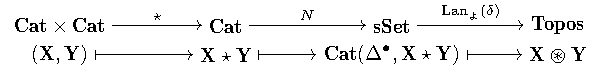
\includegraphics[scale=1]{figures/fig1}
\end{center}
\end{example}
\begin{example}[The Dold-Kan correspondence] \label{doldekanne}
The well-known Dold-Kan correspondence \cite{dold1958homology} asserts that there is an equivalence of categories between simplicial abelian groups $[\bDelta^\opp,\cate{Ab}]$ and chain complexes $\textsc{Ch}^+(\cate{Ab})$ with no negative homology, and it can be seen as an instance of the nerve\hyp{}realization paradigm.

In this case, the functor $\bDelta\to \textsc{Ch}^+(\cate{Ab})$ sending $[n]$ to $\Z^{\Delta[n]}$ (the free abelian group on $\Delta[n]$) and then to the \emph{Moore complex} $M(\Z^{\Delta[n]})$ determined by any simplicial group $A\in [\bDelta^\opp,\cate{Ab}]$ as in \cite{GoJ} is the nerve\hyp{}realization context.
\end{example}
\begin{example}[Étale spaces as Kan extensions] 
Let $X$ be a topological space, and $\cate{Opn}(X)$ its poset of open subsets. There exists a natural functor
\[
A \colon \cate{Opn}(X) \to \Top _{/X}
\]
sending $U\subseteq X$ to the same morphism $U\to X$; this works as a \textsc{nr}-context giving the pair of adjoint functors
\[
\Lan_\yon A \dashv N_A
\]
where $N_A$ is defined precisely taking the (pre)sheaf of sections of $p\in \Top _{/X}$. The resulting left adjoint is precisely the functor sending a presheaf $F\in [\cate{Opn}(X), \Sets]$ to the space whose carrier is the disjoint union of stalks $\tilde F = \coprod_{x\in X} F_x$, endowed with the final topology turning all maps of the form $\tilde s \colon U\to \tilde{F}$ sending $y$ to the equivalence class $[s]_y \in F_y$.

This adjunction restricts to an equivalence of categories between the subcategory $\cate{Sh}(X)$ of sheaves on $X$ and the subcategory $\cate{Ét}(X)$ of \emph{étale spaces} over $X$, giving a formal method to prove \cite[\athm\textbf{II.6.2}]{mac1992sheaves}. A complete proof can be found at \cite{Carche}, lectures 3 and 4.
\end{example}
\begin{example}[The tensor product of modules as a coend]
Any ring $R$ can be regarded as an $\cate{Ab}$-category with a single object, whose set of endomorphisms is the ring $R$ itself; once noticed this, we obtain natural identifications for the categories of modules over $R$:
\begin{gather*}
\cate{Mod}_R\cong {\rm Fun}(R^\opp,\cate{Ab})\\
{}_R\cate{Mod}\cong{\rm Fun}(R,\cate{Ab}).
\end{gather*}
Given $A\in \cate{Mod}_R, B\in {}_R\cate{Mod}$, we can define a functor $T_{AB}\colon R^\opp\times R\to \cate{Ab}$ which sends the unique object to the tensor product of abelian groups $A\otimes_\Z B$. The coend of this functor can be computed as the coequalizer
\[
{\rm coker}\Big( 
\xymatrix@C=2cm{
\coprod_{r\in R}A\otimes_\Z B \ar@<3pt>[r]^{r\otimes 1}\ar@<-3pt>[r]_{1\otimes r}& A\otimes_\Z B
}\Big),
\]
or in other words, there is a canonical isomorphism $\displaystyle\int^{*\in R}T_{AB}\cong A\otimes_R  B$. This point of view on tensor products can be extremely generalized (see \cite[\S \textbf{IX.6}]{McL}, but more on this has been written in \cite[\S \textbf{4}]{yoneda}): given functors $F,G\colon \C^\opp,\C\to \V$ having values in a cocomplete monoidal category, we can define the \emph{tensor product} of $F,G$ as the coend
\[
F\boxtimes_\C G:= \int^c Fc\otimes_{\V}Gc.
\]
\end{example}
\begin{remark}\label{tiaccaci}
This can be regarded as part of a general theory which defines a \textsc{thc} \emph{situation} (see \cite[\S \textbf{1.1}]{Gray1980}; these are also called \emph{adjunctions of two variables} in newer references) as a triple $\tee=(\otimes , \wedge, [\firstblank,\secondblank])$ of (bi)functors between three categories $\catS, \A, \B$, defined via the adjunctions
\[
\B(S\otimes A, B)\cong \catS(S, [A,B])\cong \A(A, S\land B).
\] 
Such an isomorphism uniquely determines the domains ant the variance of the three functors involved, in each variable; to be more clear, however, we notice that $\otimes \colon \catS\times \A\to \B$, and then $\land \colon \catS^\opp\times \B\to \A$, and $[\firstblank,\secondblank] \colon \A^\opp\times \B\to \catS$. See Exercise \textbf{3}.\refbf{ex4:lifted-thc} to show that a given \textsc{thc} situation can be lifted to one on $\catS^{\cate{I}^\opp\times \cate{J}}, \A^\cate{I}, \B^\cate{J}$ for every $\cate{I},\cate{J}\in\Cat$.
\end{remark}
To appreciate the next example we need to recall the following
\begin{proposition}\label{cofiltness}
The following properties for a functor $F\colon \C\to \Sets$ are equivalent:
\begin{itemize}
\item $F$ commutes with finite limits;
\item $\Lan_\yon F$ commutes with finite limits;
\item $F$ is a filtered colimit of representable functors;
\item The \emph{category of elements} $\elts{\C}{F}$ of $F$ (see Def\@. \refbf{eltsf} and Prop\@. \refbf{elementi}) is cofiltered.
\end{itemize}
\end{proposition}
\begin{example}[Giraud theorem using coends]
The gist of \emph{Giraud theorem} is the following statement: left exact localizations of presheaf categories $[\C^\opp, \Sets]$ classify Grothendieck toposes (\ie categories of \emph{sheaves} $\cate{Sh}(\C, J)$ with respect to a Grothendieck topology $J$).

An accessible proof of this classical representation theorem, intertwined with the theory of locally presentable categories (see for example \cite{Claudi-2006}), is contained at the end of \cite{mac1992sheaves}.
\def\E{\mathcal E}

We now try to outline an argument giving the localization between a presheaf category and a category $\E$ satisfying the axioms of Giraud, hence ``realizing'' $\E$ as a full subcategory of $[\C^\opp, \Sets]$. presheaves on $\C=\E^\text{c}\subset \E$, the subcategory of \emph{compact} object of $\E$.\footnote{An object $X\in\E$ is \emph{compact} or \emph{finitely presentable} if the hom functor $\hom(X,\firstblank)$ commutes with filtered colimits. This essentially means that $X$ can be presented with finitely many generators and relations in the ``theory'' of $\E$.}

The trick in the proof is to choose $\C$ wisely: to do this we use the fact that there is a small full subcategory $\C \subseteq \E$ of compact objects, $\E_{<\omega}$, and a full embedding $\iota\colon \C \subset \E$; this is a nerve\hyp{}realization context (\adef\refbf{nr-para}), that activates coend calculus to prove that 
\begin{enumerate}
\item The $\iota$-nerve $N_\iota$ is full and faithful and coincides with the inclusion of sheaves into presheaves $[\C^\opp,\Sets]$;
\item $\Lan_\yon\iota$ is the left exact reflection.
\end{enumerate} 
Let then
\[
\xymatrix@C=2cm{
	\Lan_\yon(\iota)\colon [\C^\opp, \Sets] \ar@<5pt>[r] & \ar@<5pt>[l]\E\colon N_\iota
}
\]
be the nerve\hyp{}realization adjunction. 

It is a matter of checking the definition, to see that the associated nerve $N_\iota$ is fully faithful, and this gives the first point: it remains then only to prove that the functor $\Lan_\yon(\iota)$ behaves like sheafification. This, in view of our characterization of the unit and counit of the nerve\hyp{}realization adjunction (Remark \refbf{unit-and-counit}) means that we have to manipulate the following chain of (iso)morphisms:
\begin{align*}
\Lan_\yon(\iota)(P) \cong & \mathcal E(\iota C, \Lan_\yon\iota(P))\\
\cong &\textstyle \mathcal E\big(\iota C, \int^A PA\times \iota A\big)\\
\leftarrow &\textstyle \int^A \mathcal E\big(\iota C, PA\times \iota A\big)\\
\cong &\textstyle \int^A PA\times \mathcal E\big(\iota C, \iota A\big)\\
\cong &\textstyle \int^A PA\times \mathcal C\big(C,A\big)\\
\cong & PC
\end{align*}
It only remains to prove that this functor is left exact. To do this we invoke \aprop\refbf{cofiltness}. It also remains to characterize \emph{sheaves} as those $P$ such that $\eta_P$ is invertible.% (this to a certain amount seems to be implied by taking only those $P$ that preserve finite limits, and yet\dots).
\end{example}
\begin{example}[Simplicial subdivision functor]\label{ex.sub}
Let again $\bDelta$ be the category of nonempty finite ordinals. The Kan $\Ex^\infty$ \emph{functor} is an endofunctor of $\sSet = [\bDelta^\opp,\Sets]$ turning every simplicial set $X$ into a \emph{Kan complex}\footnote{As defined in \cite{GoJ}, a Kan complex is a simplicial set $Y$ such that the functor $\hom(\firstblank,X)$ turns each \emph{horn inclusion} $\Lambda^k[n]\to \Delta[n]$ into an epimorphism.}. This construction is of fundamental importance in simplicial homotopy theory, and we now want to organize the classical construction in the modern terms of a nerve\hyp{}realization paradigm on $\bDelta$.

First of all, recall (\cite{GoJ}) that the nondegenerate $m$-simplices of $\Delta[n]$ are in bijective correspondence with the subsets of $\{0,\dots,n\}$ of cardinality $m+1$; this entails that the set of nondegenerate simplices of $\Delta[n]$ becomes a poset $\textsf{s}[n]$ ordered by inclusion when this partial order is tacitly transported along this bijection. We can then consider the nerve $N_\rho(\textsf{s}[n])\in\sSet$ (see Example \refbf{topnerve}). This organizes into a functor $\textsf{sd}\colon \bDelta \to \sSet$, which forms a nerve\hyp{}realization paradigm: using \aprop\refbf{nervereal} we obtain the adjunction
\begin{center}
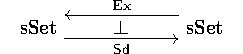
\includegraphics[scale=1]{figures/fig2}
\end{center}
where $\Ex$ is the nerve $N_\textsf{sd}$ associated to the \textsc{nr}\hyp{}paradigm $\textsf{sd}$: the set of $m$-simplices $\Ex(X)_n$ is $\sSet(\textsf{sd}(\Delta[n]), X)$.

There is a canonical map $\textsf{sd}(\Delta[n]) \to \Delta[n]$ which by precomposition and by the Yoneda lemma, induces a map $X_n=\sSet(\Delta[n],X)\xto{j^*} \sSet(\textsf{sd}(\Delta[n]),X)=\Ex(X)$, natural in $X\in\sSet$. This gives to $\Ex(\firstblank)$ the structure of a pointed functor, and in fact a \emph{well\hyp{}pointed} functor in the sense of \cite{kelly1980unified}; this, finally, means that we can define
\[
\Ex^\infty(X) \cong \varinjlim\Big( X \to \Ex(X) \to \Ex^2(X) \to \cdots\Big)
\]
as an endofunctor on $\sSet$. The functor $\Ex^\infty$ enjoys a great deal of formal properties useful in the study of simpicial homotopy theory (the most important of which is that $\Ex^\infty(X)$ is a Kan complex for each $X\in\sSet$, see \cite{GoJ}). A more intrinsic characterization of this construction is contained in \cite{ehlers2008ordinal}, and defines not only $\textsf{Sd} = \Lan_\yon\textsf{sd}$ is a Left Kan extension, but also $\textsf{sd}$: they consider the diagram of 2-cells
\begin{center}
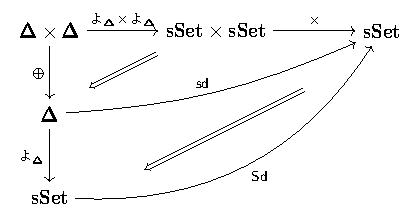
\includegraphics[scale=1]{figures/fig3}
\end{center}
where $\oplus \colon \bDelta\times\bDelta\to \bDelta$ is the \emph{ordinal sum} defined by $[m]\oplus[n] = [m+n+1]$.
% \todo[inline,caption={}]{\begin{itemize}
% \item The functor $\textsf{sd}$ is the convlution product of two Yoneda embeddings
% \item The functor $\text{Sd}$ results as a Yoneda extension.
% \end{itemize}}
\end{example}
\begin{example}[Isbell duality]\label{isbella-duella}
Isbell duality consists of the following statement: let $\V$ be a co/complete symmetric monoidal category $\V$ (this will be called a \emph{Bénabou cosmos} in the subsequent sections), and $\C \in \VCat$ a $\V$-enriched category; if we denote, as always, $[\C, \V]$ and $[\C^\opp,\V]$ the categories of covariant and contravariant functors $\C \to \V$, then we have an adjunction
\begin{center}
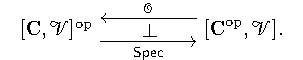
\includegraphics[scale=1]{figures/fig4}
\end{center}
This means that we find a bijection of hom-sets
\[
[\C, \V]^\opp\big( \mathcal{O}(X), Y\big) = [\C, \V]\big(Y, \mathcal{O}(X)\big)\cong [\C^\opp, \V](X, \textsf{Spec}(Y))
\]
induced by the functors
\begin{gather*}
\mathcal O \colon X \mapsto \Big( c\mapsto [\C, \V]\big(X, \yon_{\C^\opp}(c)\big)\Big)\\
\textsf{Spec}\colon Y\mapsto \Big( c \mapsto [\C,\V]^\opp\big( \yon_{\C^\opp}(c),Y \big) \Big)
\end{gather*}
Executed by an expert in coend-fu, this statement is almost a tautology thanks to \athm\refbf{naturalu}:
\begin{align*}
[\C, \V]\big(Y, \mathcal{O}(X)\big) & = \int_d \V\Big(Yd, \int_a \V(Xa, \C(a,d))\Big)\\
&\cong \int_{da}\V\big(Yd,\V(Xa, \C(a,d))\big)\\
&\cong \int_a\V\Big(Xa,\int_d\V(Yd, \C(a,d))\Big)\\
&= [\C^\opp,\V]\big(X, \textsf{Spec}(Y)\big).
\end{align*}
\end{example}
\begin{exerciseset}
\begin{exercisepoints}
\item \label{ex4:lifted-thc} Use coend-fu to show that starting from a given \textsc{thc}-situation $\tee=(\otimes , \wedge, [\firstblank,\secondblank])$, we can induce a new one $\tee' = (\boxtimes, \curlywedge, \langle\firstblank,\secondblank\rangle )$, on the categories $\catS^{\cate{I}^\opp\times \cate{J}}, \A^\cate{I}, \B^\cate{J}$, for any $\cate{I}, \cate{J}\in\Cat$; start defining $F\boxtimes G\in \B^\cate{J}$ out of $F\in \catS^{\cate{I}^\opp\times \cate{J}}, G\in \A^\cate{I}$, as the coend 
\[
\int^i F(i, \firstblank)\otimes Gi
\] 
and show that there is an adjunction
\[
{\B^\cate{J}}(F\boxtimes G, H)\cong {\catS^{\cate{I}^\opp\times \cate{J}}}(F, \langle G,H\rangle )\cong {\A^\cate{I}}(G, F\curlywedge H)
\]
for suitable functors $\langle\firstblank,\secondblank\rangle$ and $\firstblank\curlywedge\secondblank$, developing ${\B^\cate{J}}(F\boxtimes G, H) = \dots$ in two ways.
\item In this exercise $\Top$ is a nice category for algebraic topology. Define the category $\Gamma$  having objects the power-sets of finite sets, and morphisms the functions $f\colon 2^n\to 2^m$ preserving unions and set-theoretical differences.
\begin{enumerate}
\item Show that there is a functor $\bDelta\hookrightarrow \Gamma$, sending the chain  $\{0<1<\cdots<n\}$ in $\bDelta$ to $\{\varnothing\subset \{0\}\subset\cdots\subset \{0,\dots,n\}\}$ in $\Gamma$.
\item The category of presheaves of spaces $\Gamma^\opp\to \Top$ is called the category of \emph{$\Gamma$-spaces}; a $\Gamma$-space is \emph{Segal} if it turns pushout in $\Gamma$ (describe them) into homotopy pullback in $\Top$.

More explicitly, let $A\colon \Gamma^\opp\to \Top$ be a $\Gamma$-space, it is Segal if (a) $A(0)$ is contractible; (b) the canonical map $A(n)\to \prod_{i=1}^n A(1)$ is a homotopy equivalence in $\Top$.
\item Let $X\in\Top$ and $A\colon \Gamma^\opp\to \Top$; define $X\otimes A$ to be the coend (in $\Top$)
\[
\int^{n\in\Gamma} X^n\times A(n)
\] 
Show that this defines a bifunctor $\Gamma^\opp\times\Gamma\to\Top$. Show that $S^1\otimes_\Gamma A$ is homeomorphic to the geometric realization of the simplicial space $\bDelta^\opp\to \Gamma^\opp\xrightarrow{A}\Top$. If $A$ is Segal, $S^1\otimes_\Gamma A\cong BA(1)$, where $B(-)$ is the \emph{classifying space} functor.
\item Let $\C\colon \Gamma^\opp\to{\Top}\text{-}\Cat$; let $X\otimes_\Gamma \C$ be the coend (in the category of topological categories)
\[
\int^{n\in\Gamma} X^n\times \C(n).
\]
Show that $X\otimes_\Gamma (\firstblank) \colon {\Top}\text{-}\Cat\to \Cat$ commutes with finite products, namely if $\C, \D$ are topological categories, then 
\[
X\otimes_\Gamma({\C\times \D})\cong (X\otimes_\Gamma\C)\times (X\otimes_\Gamma {\bf D}).
\]
\end{enumerate}
\item Compute the $J$-realization (see Example \refbf{mordicchio}) of $X\in \cate{sSet}$ in the case $J$ is the Sierpi\'nski space $\{0 < 1\}$ with topology $\{\varnothing, J, \{1\}\}$.
\item \label{unit-and-counit} Write explicitly the unit and counit of the nerve and realization adjunction $\text{Lan}_\yon \varphi \dashv N_\varphi$.
\item Show that the nerve functor $N_\varphi$ is canonically isomorphic to $\Lan_\varphi\yon$, so that there is an adjunction
\[
\Lan_\yon\varphi \dashv \Lan_\varphi\yon.
\]
\item \label{ex:toposofic} [\awful] Example \refbf{toposophic} can be expanded and studied more deeply:
\begin{itemize}
\item Is $\odot$ a monoidal structure on $\cate{Topos}$?
\item Under which conditions on $X,Y$ is $\cate X \odot \cate Y$ equivalent to a topos of sheaves on a topological space $X \odot Y$? 
\item What are the properties of the bifunctor $(X,Y)\mapsto X \odot Y$? Does this operation resemble or extend the topological join?
\end{itemize}
\item Generalize the nerve-realization paradigm to the setting of \emph{separately cocontinuous}, or \emph{multilinear} functors. Given $\varphi \colon \C_1 \times \dots \times \C_n \to \D$, where each $\C_i$ is small and $\D$ is cocomplete, show that there exists an equivalence of categories
\[
\Cat(\C_1 \times \dots \times \C_n , \D) \cong 
\textsf{Mult}(\widehat{\C_1}\times \dots \times \widehat{\C_n}, \D)
\]
where $\textsf{Mult}(\firstblank,\secondblank)$ is the category of all functors that are cocontinuous in each variable once all the others have been fixed (hint: show it `by induction' composing multiple Kan extensions). Given $\theta \in \Cat(\C_1 \times \dots \times \C_n , \D)$, describe the right adjoint of each $\theta(c_1,\dots,c_i^\circ,\dots, c_n)\colon \widehat{\C_i} \to \D$ ($c_i^\circ$ means that all the objects $c_j$ are fixed for $j\neq i$ and $c_i\in\C$ runs free). All these functors assemble to a `vector-nerve' $N\colon \D \to \widehat{\C_1}\times \dots \times \widehat{\C_n}$.
\item Let $\yon_\C : \C \to [\C^\opp,\Sets]$ be the Yoneda embedding, and $\rotatebox[origin=c]{180}{\yon}_{\!\C} : \C^\opp\to [\C,\Sets]$ its contravariant counterpart. Show that in Example \refbf{isbella-duella} we can characterize $\mathcal{O}$ as $\Lan_{\yon_\C}(\rotatebox[origin=c]{180}{\yon}_{\!\C})$.
\end{exercisepoints}
\end{exerciseset}
